\documentclass{standalone}
\usepackage{tikz}
\usetikzlibrary{patterns, positioning}
\usepackage[sfdefault]{ClearSans} %% option 'sfdefault' activates Clear Sans as the default text font
\usepackage[T1]{fontenc}

\begin{document}
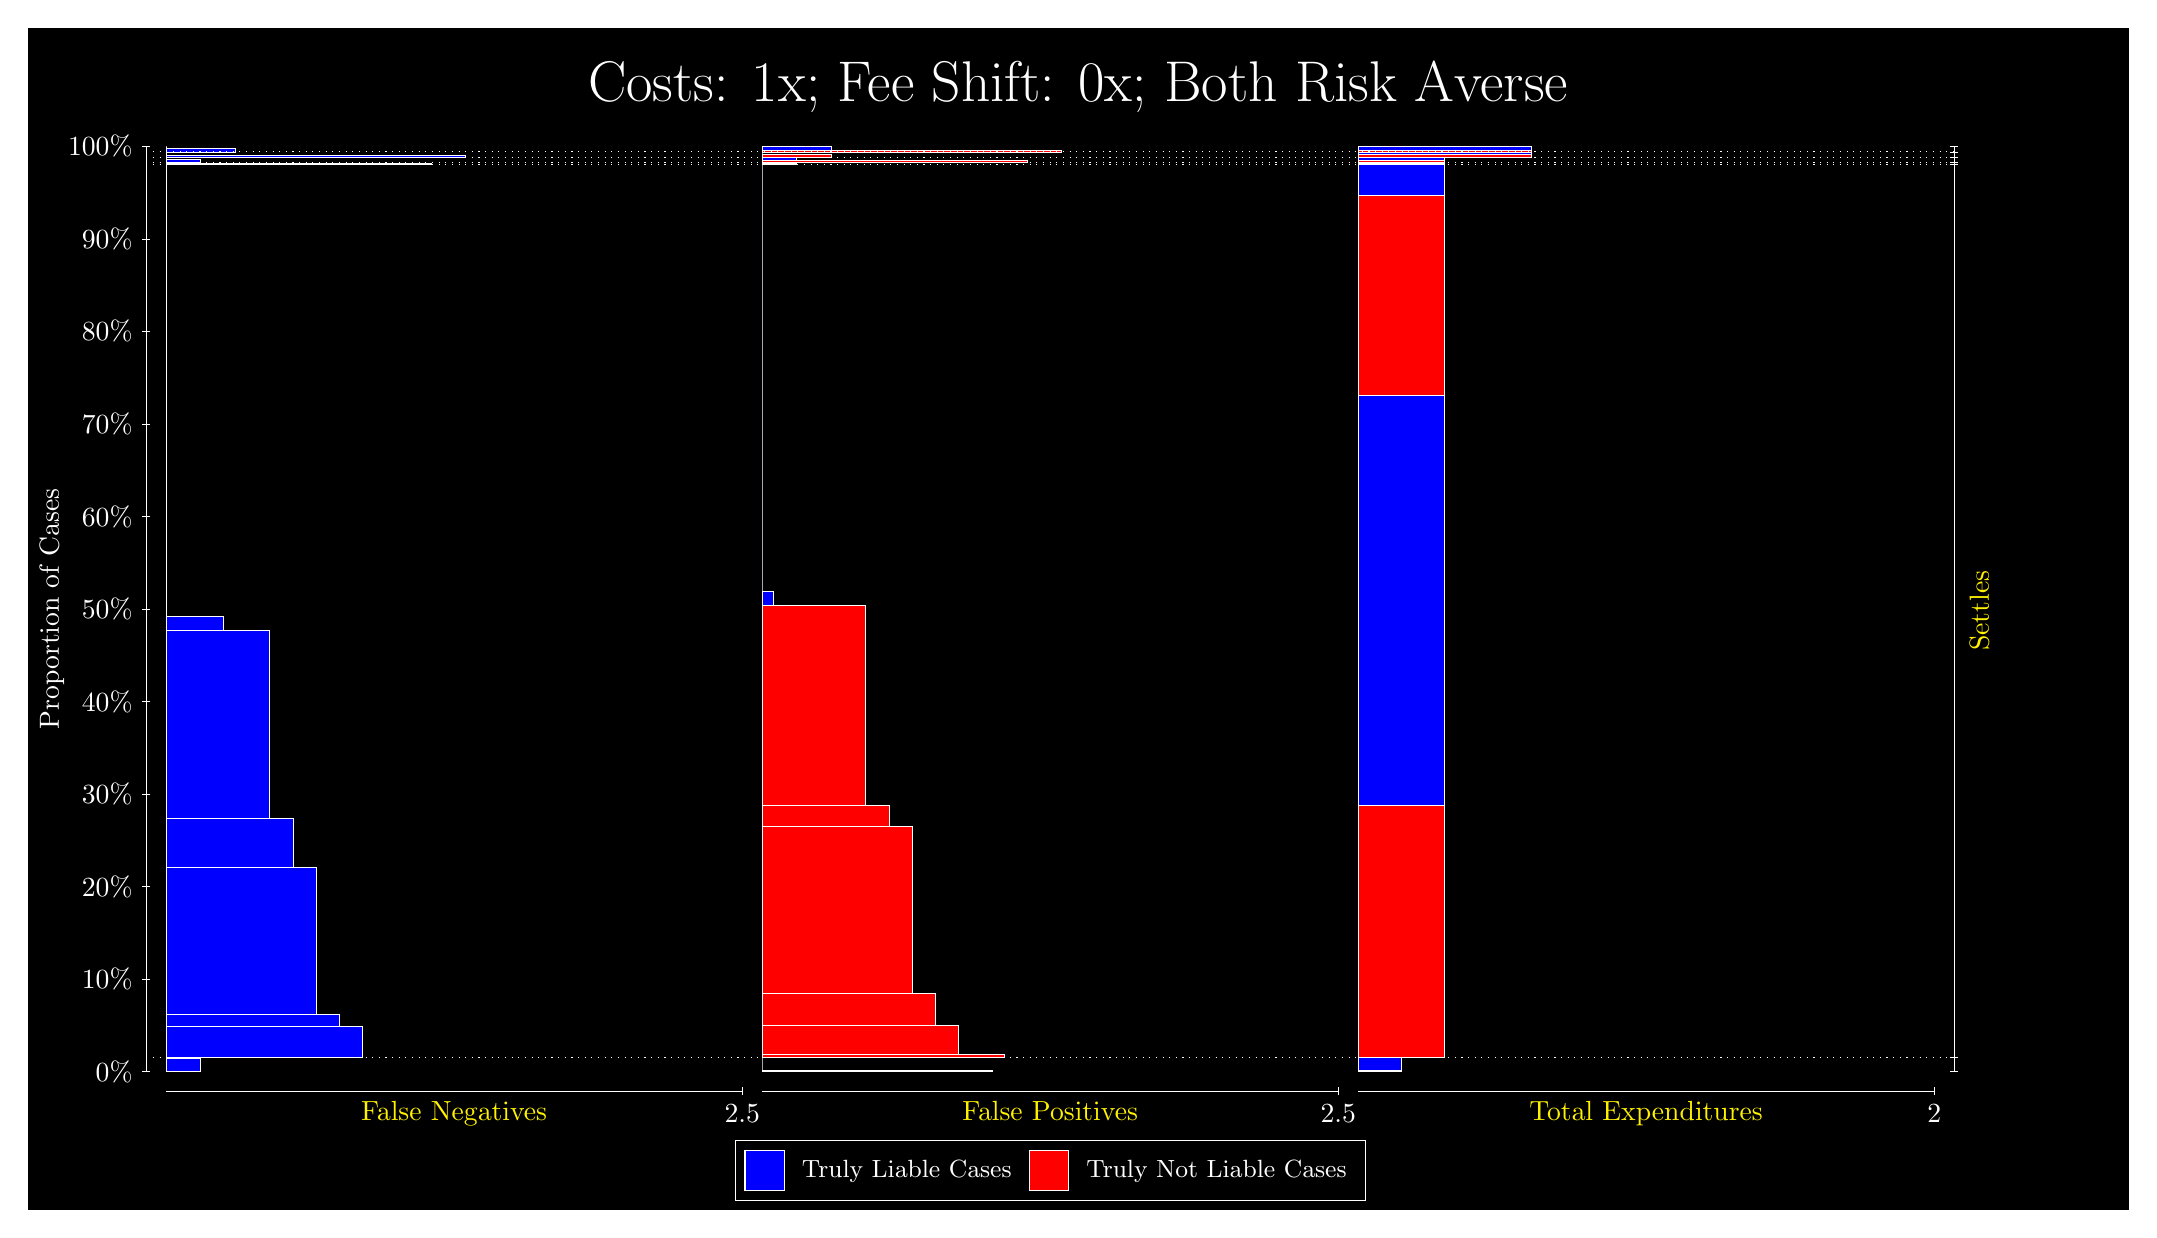
\begin{tikzpicture}
\draw[fill=black] (0,0) rectangle (26.667,15);
\draw[text=white] (0,13.5) rectangle (26.667,15) node[midway] {\huge Costs: 1x; Fee Shift: 0x; Both Risk Averse};
\draw[white, very thin] (1.5,1.75) -- (1.5,13.5);
\node[rotate=90, text=white, anchor=center] at (0.3, 7.625) {Proportion of Cases};
\draw[white, very thin] (1.45,1.75) -- (1.55,1.75);
\node[text=white, anchor=east] at (1.45, 1.75) {0\%};
\draw[white, very thin] (1.45,2.925) -- (1.55,2.925);
\node[text=white, anchor=east] at (1.45, 2.925) {10\%};
\draw[white, very thin] (1.45,4.1) -- (1.55,4.1);
\node[text=white, anchor=east] at (1.45, 4.1) {20\%};
\draw[white, very thin] (1.45,5.275) -- (1.55,5.275);
\node[text=white, anchor=east] at (1.45, 5.275) {30\%};
\draw[white, very thin] (1.45,6.45) -- (1.55,6.45);
\node[text=white, anchor=east] at (1.45, 6.45) {40\%};
\draw[white, very thin] (1.45,7.625) -- (1.55,7.625);
\node[text=white, anchor=east] at (1.45, 7.625) {50\%};
\draw[white, very thin] (1.45,8.8) -- (1.55,8.8);
\node[text=white, anchor=east] at (1.45, 8.8) {60\%};
\draw[white, very thin] (1.45,9.975) -- (1.55,9.975);
\node[text=white, anchor=east] at (1.45, 9.975) {70\%};
\draw[white, very thin] (1.45,11.15) -- (1.55,11.15);
\node[text=white, anchor=east] at (1.45, 11.15) {80\%};
\draw[white, very thin] (1.45,12.325) -- (1.55,12.325);
\node[text=white, anchor=east] at (1.45, 12.325) {90\%};
\draw[white, very thin] (1.45,13.5) -- (1.55,13.5);
\node[text=white, anchor=east] at (1.45, 13.5) {100\%};

\draw[white, very thin] (24.457,1.75) -- (24.457,13.5);
\draw[white, very thin] (24.407,1.75) -- (24.507,1.75);
\node[anchor=west] at (24.407, 1.75) {};
\draw[white, very thin] (24.407,1.9322) -- (24.507,1.9322);
\node[anchor=west] at (24.407, 1.9322) {};
\draw[white, very thin] (24.407,13.273) -- (24.507,13.273);
\node[anchor=west] at (24.407, 13.273) {};
\draw[white, very thin] (24.407,13.297) -- (24.507,13.297);
\node[anchor=west] at (24.407, 13.297) {};
\draw[white, very thin] (24.407,13.356) -- (24.507,13.356);
\node[anchor=west] at (24.407, 13.356) {};
\draw[white, very thin] (24.407,13.429) -- (24.507,13.429);
\node[anchor=west] at (24.407, 13.429) {};
\draw[white, very thin] (24.407,13.5) -- (24.507,13.5);
\node[anchor=west] at (24.407, 13.5) {};

\draw[white, very thin, fill=blue] (1.75,1.75) rectangle (2.1891,1.913);
\draw[white, very thin, fill=red] (1.75,1.913) rectangle (1.75,1.9322);
\draw[white, very thin, fill=blue] (1.75,1.9322) rectangle (4.2384,2.3271);
\draw[white, very thin, fill=blue] (1.75,2.3271) rectangle (3.9457,2.4774);
\draw[white, very thin, fill=blue] (1.75,2.4774) rectangle (3.6529,4.3409);
\draw[white, very thin, fill=blue] (1.75,4.3409) rectangle (3.3602,4.9604);
\draw[white, very thin, fill=blue] (1.75,4.9604) rectangle (3.0674,7.3595);
\draw[white, very thin, fill=blue] (1.75,7.3595) rectangle (2.4819,7.5294);
\draw[white, very thin, fill=red] (1.75,7.5294) rectangle (1.75,13.273);
\draw[white, very thin, fill=blue] (1.75,13.273) rectangle (5.1167,13.283);
\draw[white, very thin, fill=red] (1.75,13.283) rectangle (1.75,13.297);
\draw[white, very thin, fill=blue] (1.75,13.297) rectangle (2.1891,13.331);
\draw[white, very thin, fill=red] (1.75,13.331) rectangle (1.75,13.356);
\draw[white, very thin, fill=blue] (1.75,13.356) rectangle (5.5558,13.381);
\draw[white, very thin, fill=red] (1.75,13.381) rectangle (1.75,13.429);
\draw[white, very thin, fill=blue] (1.75,13.429) rectangle (2.6283,13.475);
\draw[white, very thin, fill=red] (1.75,13.475) rectangle (1.75,13.5);
\draw[white, very thin, fill=red] (9.3189,1.75) rectangle (12.246,1.7692);
\draw[white, very thin, fill=blue] (9.3189,1.7692) rectangle (9.3189,1.9322);
\draw[white, very thin, fill=red] (9.3189,1.9322) rectangle (12.393,1.9695);
\draw[white, very thin, fill=red] (9.3189,1.9695) rectangle (11.807,2.3318);
\draw[white, very thin, fill=red] (9.3189,2.3318) rectangle (11.515,2.7426);
\draw[white, very thin, fill=red] (9.3189,2.7426) rectangle (11.222,4.8647);
\draw[white, very thin, fill=red] (9.3189,4.8647) rectangle (10.929,5.1297);
\draw[white, very thin, fill=red] (9.3189,5.1297) rectangle (10.636,7.6761);
\draw[white, very thin, fill=blue] (9.3189,7.6761) rectangle (9.4652,7.846);
\draw[white, very thin, fill=blue] (9.3189,7.846) rectangle (9.3189,13.273);
\draw[white, very thin, fill=red] (9.3189,13.273) rectangle (9.758,13.287);
\draw[white, very thin, fill=blue] (9.3189,13.287) rectangle (9.3189,13.297);
\draw[white, very thin, fill=red] (9.3189,13.297) rectangle (12.686,13.321);
\draw[white, very thin, fill=blue] (9.3189,13.321) rectangle (9.758,13.356);
\draw[white, very thin, fill=red] (9.3189,13.356) rectangle (10.197,13.404);
\draw[white, very thin, fill=blue] (9.3189,13.404) rectangle (9.3189,13.429);
\draw[white, very thin, fill=red] (9.3189,13.429) rectangle (13.125,13.454);
\draw[white, very thin, fill=blue] (9.3189,13.454) rectangle (10.197,13.5);
\draw[white, very thin, fill=red] (16.888,1.75) rectangle (17.437,1.7692);
\draw[white, very thin, fill=blue] (16.888,1.7692) rectangle (17.437,1.9322);
\draw[white, very thin, fill=red] (16.888,1.9322) rectangle (17.986,5.1297);
\draw[white, very thin, fill=blue] (16.888,5.1297) rectangle (17.986,10.332);
\draw[white, very thin, fill=red] (16.888,10.332) rectangle (17.986,12.878);
\draw[white, very thin, fill=blue] (16.888,12.878) rectangle (17.986,13.273);
\draw[white, very thin, fill=red] (16.888,13.273) rectangle (17.986,13.287);
\draw[white, very thin, fill=blue] (16.888,13.287) rectangle (17.986,13.297);
\draw[white, very thin, fill=red] (16.888,13.297) rectangle (17.986,13.321);
\draw[white, very thin, fill=blue] (16.888,13.321) rectangle (17.986,13.356);
\draw[white, very thin, fill=red] (16.888,13.356) rectangle (19.083,13.404);
\draw[white, very thin, fill=blue] (16.888,13.404) rectangle (19.083,13.429);
\draw[white, very thin, fill=red] (16.888,13.429) rectangle (19.083,13.454);
\draw[white, very thin, fill=blue] (16.888,13.454) rectangle (19.083,13.5);
\draw[white, dotted] (1.5,1.9322) -- (24.457,1.9322);
\draw[white, dotted] (1.5,13.273) -- (24.457,13.273);
\draw[white, dotted] (1.5,13.297) -- (24.457,13.297);
\draw[white, dotted] (1.5,13.356) -- (24.457,13.356);
\draw[white, dotted] (1.5,13.429) -- (24.457,13.429);
\draw[white, very thin] (1.75,1.5) -- (9.0689,1.5);
\node[text=yellow, anchor=north] at (5.4094, 1.5) {False Negatives};
\draw[white, very thin] (9.0689,1.45) -- (9.0689,1.55);
\node[text=white, anchor=north] at (9.0689, 1.45) {2.5};

\draw[white, very thin] (9.3189,1.5) -- (16.638,1.5);
\node[text=yellow, anchor=north] at (12.978, 1.5) {False Positives};
\draw[white, very thin] (16.638,1.45) -- (16.638,1.55);
\node[text=white, anchor=north] at (16.638, 1.45) {2.5};

\draw[white, very thin] (16.888,1.5) -- (24.207,1.5);
\node[text=yellow, anchor=north] at (20.547, 1.5) {Total Expenditures};
\draw[white, very thin] (24.207,1.45) -- (24.207,1.55);
\node[text=white, anchor=north] at (24.207, 1.45) {2};


\node[text=yellow, centered, rotate=90] at (24.777, 7.6028) {Settles};





\draw (12.978300999999998,1.5) node[draw=none] (baseCoordinate) {};
\begin{scope}[align=center]
        \matrix[scale=0.5, draw=white, below=0.5cm of baseCoordinate, nodes={draw}, column sep=0.1cm]{
            \node[rectangle, draw, minimum width=0.5cm, minimum height=0.5cm, fill=blue] {}; &
            \node[draw=none, font=\small, text=white] (B) {Truly Liable Cases}; &
            \node[rectangle, draw, minimum width=0.5cm, minimum height=0.5cm, fill=red] {}; &
            \node[draw=none, font=\small, text=white] (B) {Truly Not Liable Cases}; \\
            };
\end{scope}

\end{tikzpicture}
\end{document}